\documentclass[border=10pt]{standalone}
\usepackage{pgfplots}
\pgfplotsset{compat=1.18}
\usepgfplotslibrary{colormaps}

\begin{document}
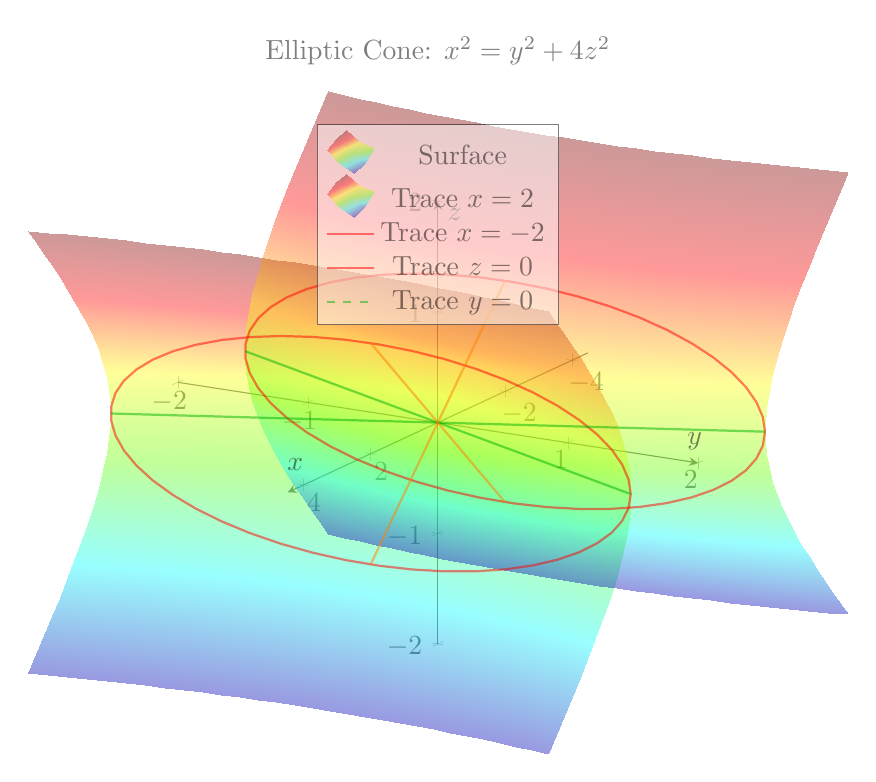
\begin{tikzpicture}
\begin{axis}[
    xlabel=$x$,
    ylabel=$y$,
    zlabel=$z$,
    title={Elliptic Cone: $x^2 = y^2 + 4z^2$},
    view={120}{20},
    axis lines=center,
    domain=-2:2,
    y domain=-2:2,
    samples=30,
    samples y=30,
    colormap/bluered,
    opacity=0.5,
    grid=major,
    width=12cm,
    height=10cm,
    legend style={at={(0.5,0.95)}, anchor=north},
]

% Surface: x = sqrt(y^2 + 4z^2)
\addplot3[surf, shader=interp, opacity=0.4, blue] ({sqrt(y^2 + 4*x^2)}, y, x);

% Surface: x = -sqrt(y^2 + 4z^2)
\addplot3[surf, shader=interp, opacity=0.4, blue] ({-sqrt(y^2 + 4*x^2)}, y, x);

% Trace x=2 (ellipse): y^2 + 4z^2 = 4
\addplot3+[domain=0:360, samples=50, red, thick, no marks] 
    ({2}, {2*cos(x)}, {sin(x)});

% Trace x=-2 (ellipse)
\addplot3+[domain=0:360, samples=50, red, thick, no marks] 
    ({-2}, {2*cos(x)}, {sin(x)});

% Trace z=0 (lines): x = +/- y
\addplot3+[domain=-2:2, samples=2, green!70!black, thick, dashed, no marks] 
    (x, x, 0);
\addplot3+[domain=-2:2, samples=2, green!70!black, thick, dashed, no marks] 
    (x, -x, 0);

% Trace y=0 (lines): x = +/- 2z
\addplot3+[domain=-1:1, samples=2, orange, thick, dashdotted, no marks] 
    (2*x, 0, x);
\addplot3+[domain=-1:1, samples=2, orange, thick, dashdotted, no marks] 
    (-2*x, 0, x);

\legend{Surface, Trace $x=2$, Trace $x=-2$, Trace $z=0$, Trace $y=0$}

\end{axis}
\end{tikzpicture}
\end{document}